% !TeX program = xelatex
\documentclass[a4paper]{article}

\input{style/ch_xelatex.tex}
\input{style/scala.tex}

%代码段设置
\lstset{numbers=left,
	basicstyle=\tiny,
	numberstyle=\tiny,
	keywordstyle=\color{blue!70},
	commentstyle=\color{red!50!green!50!blue!50},
	frame=single, rulesepcolor=\color{red!20!green!20!blue!20},
	escapeinside=``
}

\graphicspath{ {images/} }
\usepackage{ctex}
\usepackage{graphicx}
\usepackage{color,framed}%文本框
\usepackage{listings}
\usepackage{caption}
\usepackage{amssymb}
\usepackage{enumerate}
\usepackage{xcolor}
\usepackage{bm} 
\usepackage{lastpage}%获得总页数
\usepackage{fancyhdr}
\usepackage{tabularx}  
\usepackage{geometry}
\usepackage{minted}
\usepackage{graphics}
\usepackage{subfigure}
\usepackage{float}
\usepackage{pdfpages}
\usepackage{pgfplots}
\pgfplotsset{width=10cm,compat=1.9}
\usepackage{multirow}
\usepackage{footnote}
\usepackage{booktabs}

%------------------------代码-------------------
\usepackage{xcolor} 
\usepackage{listings} 
\lstset{ 
	language=Verilog, % 设置默认语言为Verilog
	breaklines,%自动换行
	basicstyle=\small\ttfamily, % 使用等宽字体
	escapeinside=``,
	keywordstyle=\color{ blue!70} \bfseries,
	commentstyle=\color{red!50!green!50!blue!50},% 
	stringstyle=\ttfamily,% 
	extendedchars=false,% 
	linewidth=\textwidth,% 
	numbers=left,% 
	numberstyle=\tiny \color{blue!50},% 
	frame=trbl,% 
	rulesepcolor= \color{ red!20!green!20!blue!20} 
}

%-------------------------页面边距--------------
\geometry{a4paper,left=2.3cm,right=2.3cm,top=2.7cm,bottom=2.7cm}
%-------------------------页眉页脚--------------
\usepackage{fancyhdr}
\pagestyle{fancy}
\lhead{\kaishu \leftmark}
% \chead{}
\rhead{\kaishu 计算机组成原理实验报告}%加粗\bfseries 
\lfoot{}
\cfoot{\thepage}
\rfoot{}
\renewcommand{\headrulewidth}{0.1pt}  
\renewcommand{\footrulewidth}{0pt}%去掉横线
\newcommand{\HRule}{\rule{\linewidth}{0.5mm}}%标题横线
\newcommand{\HRulegrossa}{\rule{\linewidth}{1.2mm}}
\setlength{\textfloatsep}{10mm}%设置图片的前后间距
%--------------------文档内容--------------------

\begin{document}
	\renewcommand{\contentsname}{目\ 录}
	\renewcommand{\appendixname}{附录}
	\renewcommand{\appendixpagename}{附录}
	\renewcommand{\refname}{参考文献} 
	\renewcommand{\figurename}{图}
	\renewcommand{\tablename}{表}
	\renewcommand{\today}{\number\year 年 \number\month 月 \number\day 日}
	
	%-------------------------封面----------------
	\begin{titlepage}
		\begin{center}
			
\includegraphics[width=0.8\textwidth]{NKU.png}\\[1cm]
			\vspace{20mm}
			\textbf{\huge\textbf{\kaishu{计算机学院}}}\\[0.5cm]
			\textbf{\huge{\kaishu{计算机体系结构实验报告}}}\\[2.3cm]
			\textbf{\Huge\textbf{\kaishu{五级流水复习和分析}}}
			
			\vspace{\fill}
			
			% \textbf{\Large \textbf{计算机体系结构实验报告}}\\[0.8cm]
			% \HRule \\[0.9cm]
			% \HRule \\[2.0cm]
			\centering
			\textsc{\LARGE \kaishu{姓名\ :\ 王一诺}}\\[0.5cm]
			\textsc{\LARGE \kaishu{学号\ :\ 2312331}}\\[0.5cm]
			\textsc{\LARGE \kaishu{专业\ :\ 计算机科学与技术}}\\[0.5cm]
			\textsc{\LARGE \kaishu{指导老师\ :\ 董前琨}}\\[0.5cm]
			
			\vfill
			{\Large \today}
		\end{center}
	\end{titlepage}
	
	\renewcommand {\thefigure}{\thesection{}.\arabic{figure}}%图片按章标号
	\renewcommand{\figurename}{图}
	\renewcommand{\contentsname}{目录}  
	\cfoot{\thepage\ of \pageref{LastPage}}%当前页 of 总页数
	
	
	% 生成目录
	\clearpage
	\tableofcontents
	\newpage
	\setcounter{figure}{0} % 每章开始前重置图片计数器
	
	\section{实验目的}
	本次实验旨在通过对一个已有的五级流水线CPU源码进行bug修改、分析和调试，实现以下目标：
	\begin{enumerate}
		\item 深入理解五级流水线（IF、ID、EX、MEM、WB）的工作原理、数据通路和控制逻辑。
		\item 熟悉并掌握流水线 CPU 的原理和设计。
		\item 通过修复源码中的Bug，提升Verilog代码调试能力和对CPU内部复杂控制信号交互的理解。
		\item 参考MIPS指令集，对新增指令进行具体分析，包括运算、乘除、转移和访存四类指令，从而全面掌握指令在流水线各阶段的实现细节。
		\item 培养对 CPU 设计的兴趣，加深对 CPU 现有架构的理解和深思。
	\end{enumerate}
	
	\section{实验要求}
	请参考实验指导手册，完成五级流水线CPU工程的顺利运行，完成如下工作：
	
	1、修改原始代码source code中的bug，保证指令运行正确
	
	2、针对五级流水线中新增加的指令，逐级分析指令执行过程和执行结果，梳理流水线知识点
	
	3、将上述两部分内容写入实验报告提交。
	
	\section{实验原理图}
	\setcounter{figure}{0}
	本实验中实现的五级流水线CPU，其核心数据通路和控制单元如下图所示。CPU将指令执行过程划分为取指（FETCH）、译码（DECODE）、执行（EXE）、访存（MEM）和写回（WB）五个阶段，并通过四级流水线寄存器（IF/ID, ID/EXE, EXE/MEM, MEM/WB）在阶段间传递数据和控制信号。
	\begin{figure}[H]
		\centering
		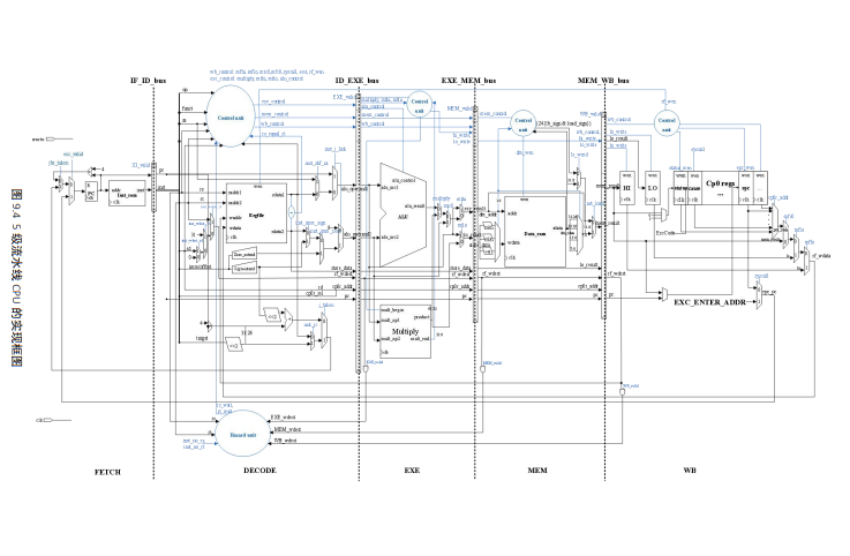
\includegraphics[width=\textwidth]{placeholder.png}
		\caption{五级流水线CPU详细框图}
		\label{fig:pipeline_detailed}
	\end{figure}
	
	一个更简化的静态模型如下，它清晰地展示了各阶段与主要部件（指令ROM、寄存器堆、数据RAM）的交互关系。
	\begin{figure}[H]
		\centering
		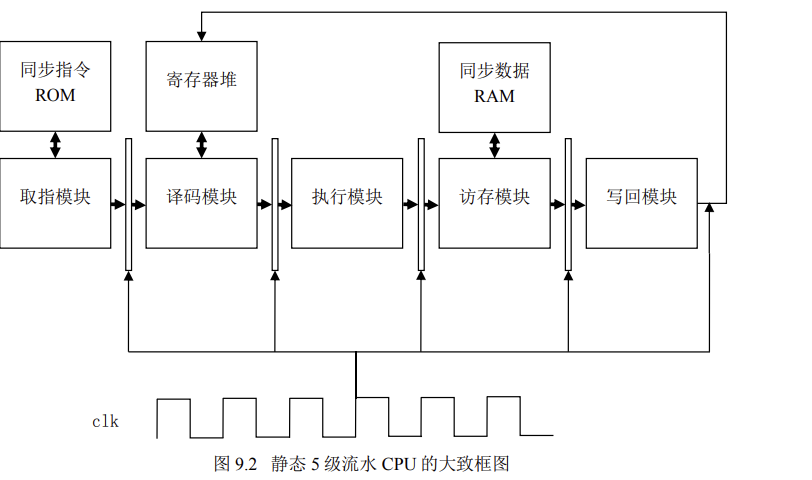
\includegraphics[width=0.8\textwidth]{placeholder2.png}
		\caption{静态五级流水CPU功能框图}
		\label{fig:pipeline_static}
	\end{figure}
	
	\section{现有流水线问题分析}
	尝试对source\_code进行仿真，波形图如下：
	\begin{figure}[H]
		\centering
		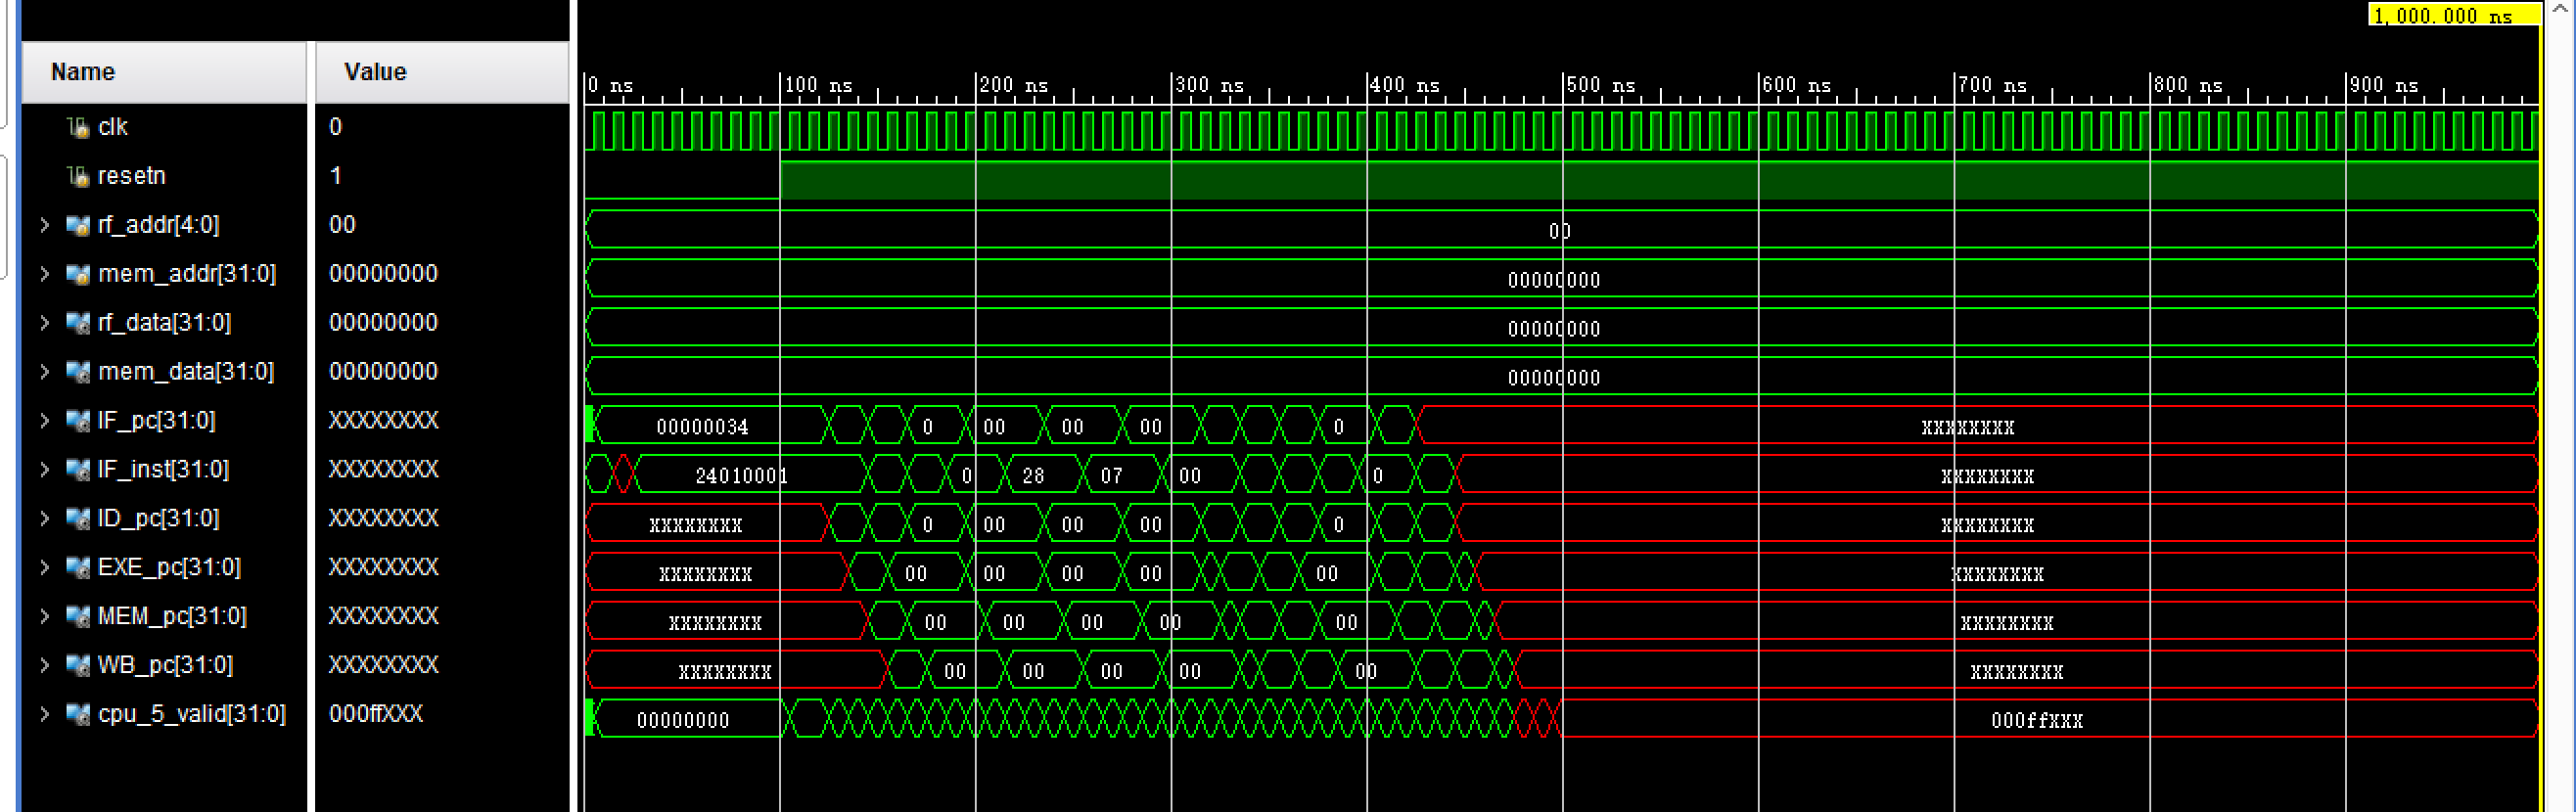
\includegraphics[width=\textwidth]{wrong.png}
		\caption{源代码错误仿真波形}
		\label{fig:wrong}
	\end{figure}
	
	经过分析，发现是指令ROM的读取延迟与IF\_over信号生成时机的不匹配导致的。有两种方案解决该问题：
	\subsection{取消 Primitives Output Register}
	在配置IP核时，取消勾选Primitives Output Register的选项，如下图所示：
	\begin{figure}[H]
		\centering
		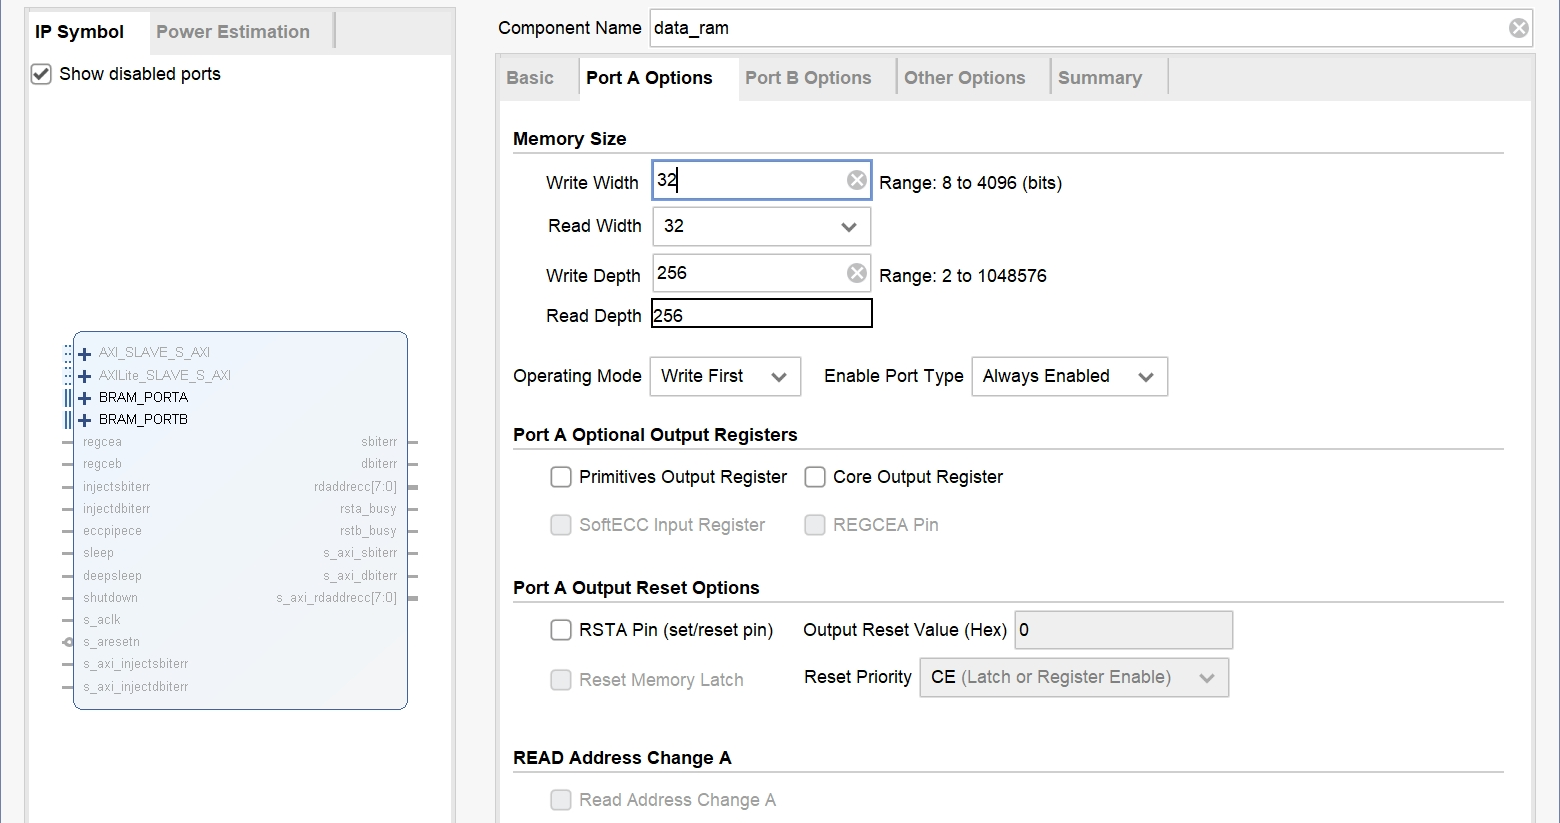
\includegraphics[width=\textwidth]{ramip.png}
		\caption{修改data\_ram}
		\label{fig:ramip}
	\end{figure}
	\begin{figure}[H]
		\centering
		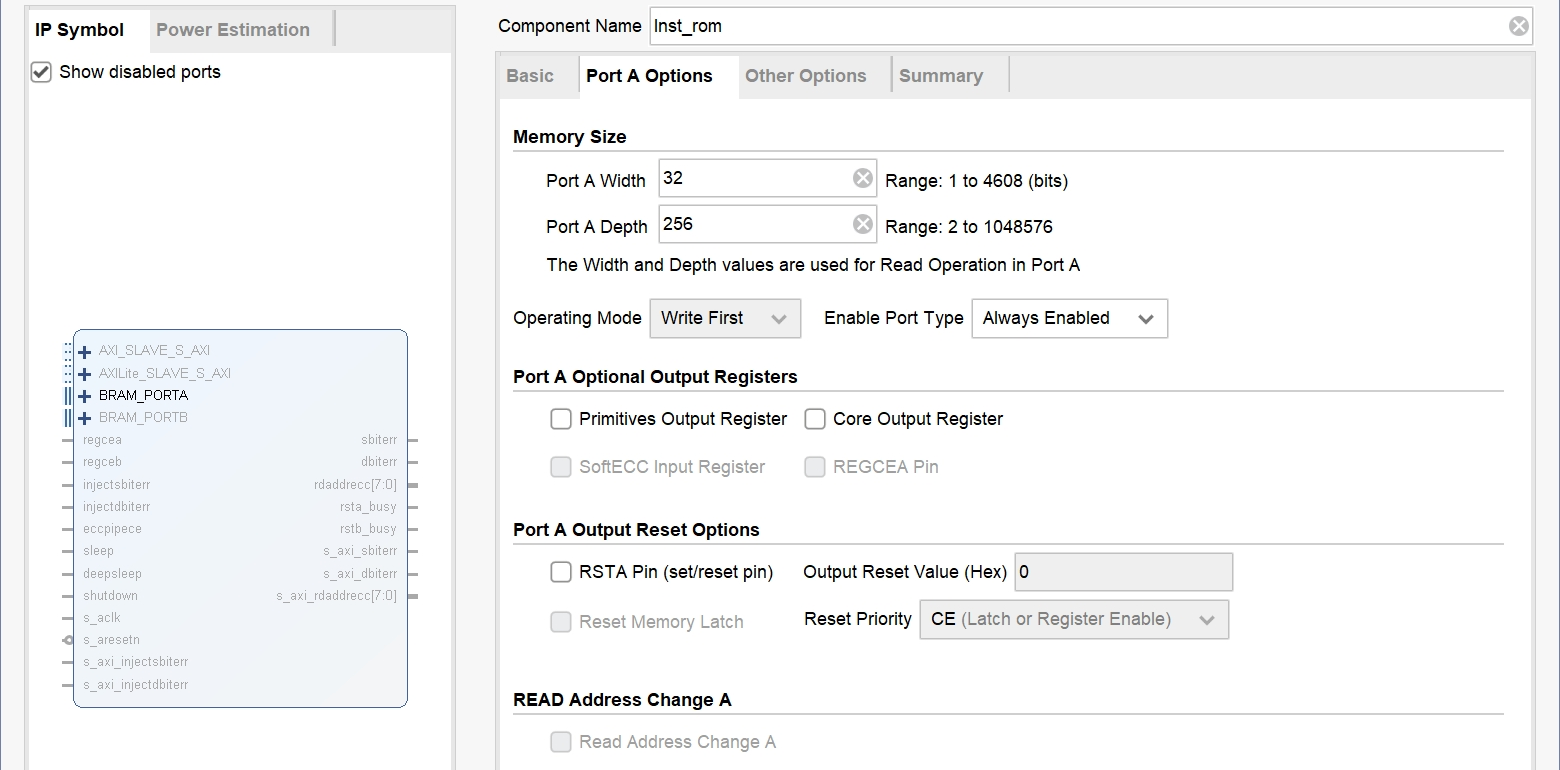
\includegraphics[width=\textwidth]{romip.png}
		\caption{修改inst\_rom}
		\label{fig:romip}
	\end{figure}
	
	勾选此选项时：IP核在BRAM原语输出端额外增加一级寄存器;
	
	取消勾选后：只有BRAM内部的地址寄存器。使ROM变成真正的单周期延迟，保证“取数据时，有一拍延时”，让IF\_over信号与指令数据真正可用的时刻同步。
	
	\subsection{修改 IF\_over 逻辑}
	找到fetch.v中的IF执行逻辑：
	\begin{lstlisting}[caption={fetch.v-old}]
	//-----{IF执行完成}begin
		//由于指令rom为同步读写的,
		//取数据时，有一拍延时
		//即发地址的下一拍时钟才能得到对应的指令
		//故取指模块需要两拍时间
		//故每次PC刷新，IF_over都要置0
		//然后将IF_valid锁存一拍即是IF_over信号
		always @(posedge clk)
		begin
			if (!resetn || next_fetch)
			begin
				IF_over <= 1'b0;
			end
			else
			begin
				IF_over <= IF_valid;
			end
		end
		//如果指令rom为异步读的，则IF_valid即是IF_over信号，
		//即取指一拍完成
	//-----{IF执行完成}end
	\end{lstlisting}
	修改为：
	\begin{lstlisting}[caption={fetch.v-new}]
		reg temp;
		always @(posedge clk)
		begin
			if (!resetn || next_fetch)
			begin
				IF_over <= 1'b0;
				temp<=1'b0;
			end
			else if(!temp)
			begin
				temp<=1'b1;
			end
			else
			begin
				IF_over <= IF_valid;
			end
		end
	\end{lstlisting}
	这样，通过temp信号增加1拍等待，即通过软件逻辑补偿额外的1拍延迟，使IF\_over信号与数据真正可用时刻对齐。
	
	\subsection{总结修改逻辑}
	
	两种方案殊途同归：都让IF\_over信号与指令数据真正可用的时刻同步
	\begin{enumerate}
		\item 方案1：让硬件适配代码假设（1拍延迟）
		\item 方案2：让代码适配硬件现实（2拍延迟）
	\end{enumerate}
	\begin{table}[!htbp]
		\centering
		\begin{tabular}{ccc}
			\toprule  
			维度& 方案1（硬件配置）& 方案2（代码逻辑）\\
			\midrule
			修改对象& IP核配置& Verilog控制逻辑\\
			ROM延迟& 2拍→1拍& 保持2拍\\
			IF\_over时机& 保持原逻辑& 延后1拍\\
			本质& 消除硬件多余延迟& 适配硬件实际延迟\\
			\bottomrule
		\end{tabular}
		\caption{对比总结}
		\label{table:t1}
	\end{table}
	
	修改后：
	\begin{figure}[H]
		\centering
		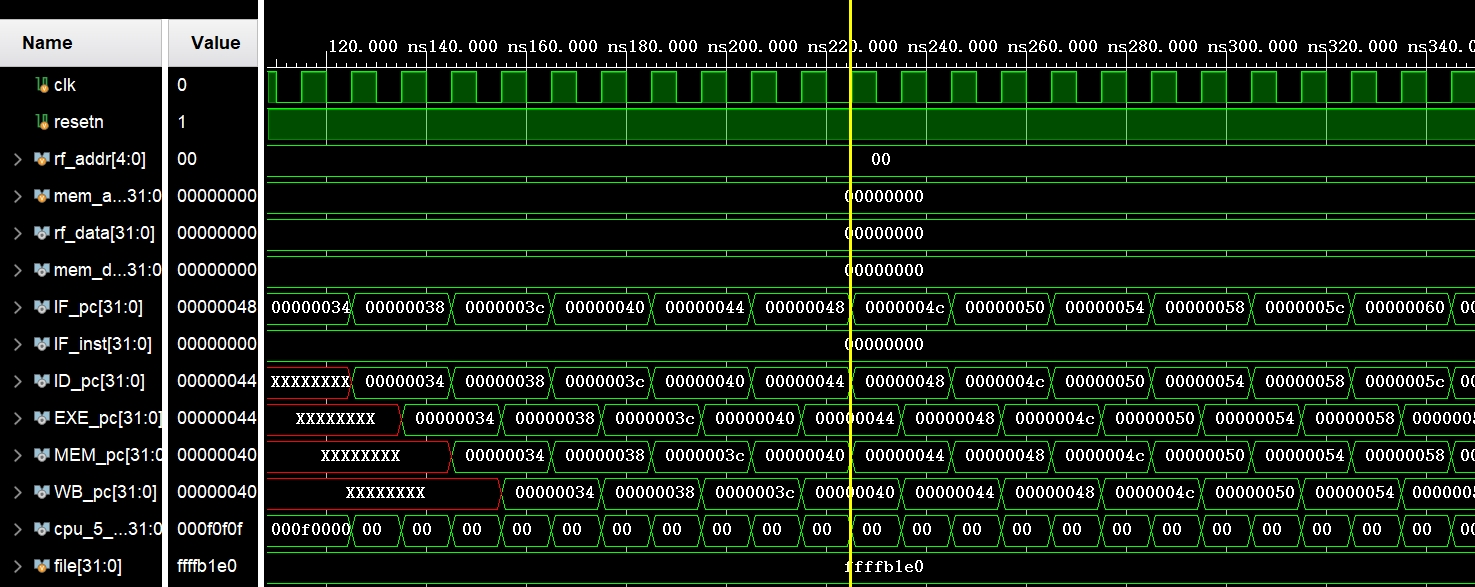
\includegraphics[width=\textwidth]{fixed.png}
		\caption{改后仿真波形}
		\label{fig:fixed}
	\end{figure}
	
	\section{新增加指令分析}
	根据实验指导书附录，该实验新增了9条指令，接下来我将结合对应具体代码逐级分析指令执行过程和执行结果。
	\subsection{MULT（乘法指令）}
	\paragraph{指令概述与功能}
	MULT指令是MIPS架构中的有符号乘法指令，它将两个32位有符号整数相乘，产生一个64位的有符号乘积。乘积的高32位存储在HI寄存器中，低32位存储在LO寄存器中。这是一条R型指令，指令格式为000000\_sssss\_ttttt\_00000\_00000\_011000，其中rs和rt字段指定两个源操作数寄存器，rd和sa字段必须为0，功能码funct为011000。
	\paragraph{IF级（取指阶段）}
	相关代码：
	\begin{lstlisting}[caption={IF}]
		// fetch.v
		// 从指令存储器读取MULT指令
		assign inst_addr = pc;  // 将PC送到指令ROM
		// 下一周期得到指令: 000000_sssss_ttttt_00000_00000_011000
	\end{lstlisting}
	
	在取指阶段，程序计数器PC保存着当前MULT指令的地址。这个地址通过inst\_addr信号线被送到指令ROM模块。由于实验中使用的是同步读写的指令存储器，地址在当前时钟周期的上升沿被锁存到ROM中，实际的指令数据要到下一个时钟周期才能读出。在这个等待期间，IF\_over信号保持为低电平，表示取指尚未完成。
	
	PC的计算遵循特定的优先级规则。首先检查是否有异常发生，如果exc\_valid信号有效，PC将跳转到异常入口地址。其次检查是否有分支跳转，如果jbr\_taken信号有效，PC将跳转到jbr\_target指定的目标地址。如果都不满足，PC就简单地加4指向下一条顺序指令。这个next\_pc的计算是组合逻辑，但实际更新PC寄存器要等到next\_fetch信号有效时，这个信号实际上就是IF\_allow\_in信号。
	对于MULT指令来说，它本身不是跳转指令，所以在正常情况下会按顺序取指。指令存储器在下一个周期返回32位的指令编码，此时IF\_over信号变为高电平，表示取指完成。IF模块将PC值和指令inst打包成64位的IF\_ID\_bus信号，准备传递给译码阶段。
	\paragraph{ID级（译码阶段）}
	相关代码：
	\begin{lstlisting}[caption={ID}]
		// decode.v
		// 指令识别
		assign inst_MULT = op_zero & (rd==5'd0) & sa_zero & (funct == 6'b011000);
		
		// 设置控制信号
		assign multiply = inst_MULT;  // 乘法标志置1
		
		// ALU操作数准备
		assign alu_operand1 = rs_value;  // 第一个乘数
		assign alu_operand2 = rt_value;  // 第二个乘数
		
		// 写回控制
		assign rf_wen = 1'b0;  // MULT不直接写回寄存器
		assign rf_wdest = 5'd0;
		
		// 数据相关检测
		assign rs_wait = (rs!=5'd0) & ((rs==EXE_wdest) | (rs==MEM_wdest) | (rs==WB_wdest));
		assign rt_wait = (rt!=5'd0) & ((rt==EXE_wdest) | (rt==MEM_wdest) | (rt==WB_wdest));
		
		// ID_EXE总线打包
		assign ID_EXE_bus = {multiply,      // 1'b1
			mthi, mtlo,    // 都为0
			alu_control,   // 12'b0
			alu_operand1,  // rs_value
			alu_operand2,  // rt_value
			...};
	\end{lstlisting}
	
	译码阶段接收到IF\_ID\_bus\_r锁存的数据，这包含了PC值和32位指令编码。译码器首先将指令分解为各个字段：操作码op、源寄存器rs和rt、目标寄存器rd、移位量sa、功能码funct等。对于MULT指令，译码器检测到op字段全为0，rd字段为0，sa字段为0，且funct字段等于011000，因此inst\_MULT信号被置为高电平。
	
	MULT指令的识别逻辑要求op为0（表示R型指令），rd为0（因为MULT不直接写通用寄存器），sa为0（MULT不使用移位量），funct等于011000。
	
	一旦识别出MULT指令，译码器就开始设置各种控制信号。multiply信号被置为1，这是一个关键信号，它会一直传递到执行阶段，告诉乘法器模块开始工作。mthi和mtlo信号都为0，因为MULT本身不是直接向HI/LO写入的指令，而是通过乘法运算的结果自动更新这两个寄存器。
	
	ALU控制信号alu\_control的12位全部为0，因为MULT指令不需要使用ALU进行任何算术或逻辑运算。ALU的作用在MULT指令中被完全旁路了。然而，alu\_operand1和alu\_operand2仍然需要设置，它们分别被赋值为rs\_value和rt\_value，也就是从寄存器堆读出的两个源操作数的值。这两个操作数会被传递到执行阶段，供乘法器使用。
	
	寄存器堆的读取是通过rs和rt信号完成的，这两个信号直接来自指令的相应字段。寄存器堆是异步读的，所以在同一个周期内，只要给出地址，就能得到数据。rs\_value和rt\_value就是读出的结果。但是这里有一个数据相关性的问题。
	
	数据相关性检测是译码阶段的核心功能之一。如果MULT指令需要读取的rs或rt寄存器正好是前面某条还在流水线中执行的指令要写回的目标寄存器，那么就存在数据相关。具体来说，rs\_wait信号会检查rs是否等于EXE\_wdest、MEM\_wdest或WB\_wdest中的任何一个。如果相等且rs不为0号寄存器，rs\_wait就会置为1。rt\_wait的检测逻辑类似。
	
	当存在数据相关时，ID\_over信号会保持为0，阻止指令向下一级流水。这实际上是一种流水线停顿机制。译码阶段会一直等待，直到前面的指令完成写回，数据相关解除，EXE\_wdest、MEM\_wdest或WB\_wdest中不再包含rs或rt，此时rs\_wait和rt\_wait都变为0，ID\_over才会变为1，允许MULT指令进入执行阶段。
	
	对于MULT指令，rf\_wen被设置为0，rf\_wdest被设置为0，因为MULT不写通用寄存器堆。它的结果会写入HI和LO这两个特殊寄存器。mem\_control信号全为0，表示不进行内存访问。store\_data无效，因为不需要存储。
	
	所有这些控制信号和数据被打包成167位的ID\_EXE\_bus。这个总线包含了执行阶段需要的所有信息：multiply标志、mthi/mtlo标志（都为0）、alu\_control（全0）、两个乘数operand1和operand2、内存控制信号、写回控制信号、以及PC值。当ID\_over和EXE\_allow\_in都为1时，ID\_EXE\_bus的内容会在时钟上升沿被锁存到ID\_EXE\_bus\_r寄存器中，供执行阶段使用。
	\paragraph{EXE级（执行阶段）}
	相关代码：
	\begin{lstlisting}[caption={EXE}]
		// exe.v
		// 解包总线
		assign {multiply, mthi, mtlo, alu_control, 
			alu_operand1, alu_operand2, ...} = ID_EXE_bus_r;
		
		// 启动乘法器
		assign mult_begin = multiply & EXE_valid;
		
		// multiply.v - 乘法器模块
		// 1. 计算操作数符号和绝对值
		assign op1_sign = mult_op1[31];
		assign op2_sign = mult_op2[31];
		assign op1_absolute = op1_sign ? (~mult_op1+1) : mult_op1;
		assign op2_absolute = op2_sign ? (~mult_op2+1) : mult_op2;
		
		// 2. 加载被乘数和乘数（第一个周期）
		always @(posedge clk) begin
		if (mult_begin) begin
		multiplicand <= {32'd0, op1_absolute};  // 低32位
		multiplier <= op2_absolute;
		product_temp <= 64'd0;
		mult_valid <= 1'b1;
		end
		end
		
		// 3. 迭代计算（多个周期）
		always @(posedge clk) begin
		if (mult_valid) begin
		multiplicand <= {multiplicand[62:0], 1'b0};  // 左移
		multiplier <= {1'b0, multiplier[31:1]};      // 右移
		product_temp <= product_temp + partial_product;
		end
		end
		
		assign partial_product = multiplier[0] ? multiplicand : 64'd0;
		
		// 4. 乘法结束检测
		assign mult_end = mult_valid & ~(|multiplier);  // 乘数全0时结束
		
		// 5. 结果符号处理
		assign product = product_sign ? (~product_temp+1) : product_temp;
		
		// EXE完成控制
		assign EXE_over = EXE_valid & (~multiply | mult_end);  // 等待乘法完成
		
		// 准备写HI/LO的数据
		assign exe_result = multiply ? product[63:32] : alu_result;  // HI
		assign lo_result = product[31:0];                             // LO
		assign hi_write = multiply;  // 写HI使能
		assign lo_write = multiply;  // 写LO使能
		
		// EXE_MEM总线打包
		assign EXE_MEM_bus = {mem_control,   // 4'b0
			store_data,    // 无效
			exe_result,    // 高32位乘积
			lo_result,     // 低32位乘积
			hi_write,      // 1'b1
			lo_write,      // 1'b1
			mfhi, mflo,    // 都为0
			...};
	\end{lstlisting}
	
	执行阶段从ID\_EXE\_bus\_r中解包出所有控制信号和数据。对于MULT指令，关键的信号是multiply为1，alu\_operand1和alu\_operand2包含了两个要相乘的数。
	
	执行阶段首先生成mult\_begin信号，这个信号等于multiply与EXE\_valid的逻辑与。只有当执行级有效且multiply为1时，乘法才会真正开始。mult\_begin信号被送到乘法器模块multiply\_module，触发乘法运算的启动。
	
	乘法器模块的设计采用了迭代累加算法，这是一种低效率但实现简单的算法。首先，乘法器需要处理操作数的符号。两个源操作数mult\_op1和mult\_op2可能是负数，乘法器提取它们的符号位op1\_sign和op2\_sign（即最高位），然后计算绝对值。对于正数，绝对值就是它本身；对于负数，绝对值是取反加1的结果。这样，op1\_absolute和op2\_absolute就得到了两个操作数的绝对值。
	
	在mult\_begin信号到来的那个时钟周期，乘法器进行初始化。multiplicand寄存器被加载为{32'd0 , op1\_absolute}，这是一个64位的值，低32位是第一个操作数的绝对值，高32位全0。multiplier寄存器被加载为op2\_absolute，这是一个32位的值。product\_temp寄存器被清零，它将用于累加部分积。mult\_valid寄存器被置为1，表示乘法正在进行。
	
	从下一个时钟周期开始，乘法器进入迭代循环。每个周期，乘法器检查multiplier的最低位。如果这一位是1，说明当前的被乘数需要累加到部分积中，所以partial\_product等于multiplicand；如果这一位是0，partial\_product就是0。product\_temp在每个周期累加partial\_product。
	
	同时，multiplicand每周期逻辑左移一位，相当于乘以2。这对应了乘法的原理：如果乘数的某一位是1，被乘数要左移相应的位数后累加。multiplier每周期逻辑右移一位，这样下一个周期就会检查下一位。
	
	这个迭代过程一直持续到multiplier的所有位都变成0为止。此时mult\_end信号变为1，mult\_end的条件是mult\_valid为1且multiplier的所有位都是0（用或归约运算符检测）。当mult\_end为1时，mult\_valid在下一个周期被清零，表示乘法结束。
	
	在整个乘法过程中，product\_sign寄存器记录了乘积的符号，它等于两个操作数符号的异或。如果两个操作数同号，product\_sign为0，乘积为正；如果异号，product\_sign为1，乘积为负。
	
	乘法结束后，最终的product是根据符号调整的。如果product\_sign为1，product等于product\_temp取反加1（即取补码）；如果为0，product直接等于product\_temp。这个64位的product就是最终的乘法结果。
	
	在执行阶段，EXE\_over信号的生成逻辑需要特别注意。对于普通的ALU指令，一个周期就能完成，所以EXE\_over可以直接等于EXE\_valid。但对于MULT指令，需要等待多个周期直到乘法完成。因此，EXE\_over的逻辑是：EXE\_valid与（非multiply或mult\_end）的逻辑与。这意味着，如果不是乘法指令，立即完成；如果是乘法指令，必须等到mult\_end为1才完成。这个设计确保了流水线能够正确地停顿等待乘法结果。
	
	exe\_result的选择逻辑也很重要。对于MULT指令，exe\_result应该选择product的高32位，即product[63:32]，这将被写入HI寄存器。lo\_result选择product的低32位，即product[31:0]，这将被写入LO寄存器。hi\_write和lo\_write信号都被置为1，表示需要更新HI和LO寄存器。
	
	所有这些信息被打包进EXE\_MEM\_bus。这个154位的总线包含：内存控制信号（全0，不访问内存）、store\_data、exe\_result（product高32位）、lo\_result（product低32位）、hi\_write（1）、lo\_write（1）、其他控制信号、以及PC值。
	\paragraph{MEM级（访存阶段）}
	相关代码：
	\begin{lstlisting}[caption={MEM}]
		// mem.v
		// MULT指令不访问内存，直接传递
		assign {mem_control, store_data, exe_result, lo_result,
			hi_write, lo_write, ...} = EXE_MEM_bus_r;
		
		assign inst_load = 1'b0;
		assign inst_store = 1'b0;
		assign dm_wen = 4'b0000;  // 不写内存
		
		// MEM立即完成
		assign MEM_over = MEM_valid;  // 非load指令一拍完成
		
		// 传递到WB
		assign mem_result = exe_result;  // 高32位
		assign MEM_WB_bus = {rf_wen,      // 1'b0
			rf_wdest,    // 5'd0
			mem_result,  // 高32位
			lo_result,   // 低32位
			hi_write,    // 1'b1
			lo_write,    // 1'b1
			...};
	\end{lstlisting}
	
	访存阶段对于MULT指令来说相对简单，因为MULT不涉及内存访问。MEM模块从EXE\_MEM\_bus\_r中解包数据，检查mem\_control信号，发现inst\_load和inst\_store都为0，说明不需要访问数据RAM。因此，dm\_wen被设置为4'b0000，不写内存；dm\_addr和dm\_wdata的值无关紧要，因为它们不会被使用。
	
	MEM\_over信号的生成依赖于是否有load操作。对于load指令，由于数据RAM是同步读的，需要两个周期才能拿到数据，所以MEM\_over需要等待。但对于MULT指令，inst\_load为0，MEM\_over直接等于MEM\_valid，意味着访存阶段一个周期就完成了。
	
	mem\_result的选择逻辑中，由于inst\_load为0，mem\_result直接等于exe\_result，也就是乘积的高32位。这个值将传递到写回阶段。
	
	MEM\_WB\_bus将所有需要的信息打包传递给写回阶段：rf\_wen（0）、rf\_wdest（0）、mem\_result（乘积高32位）、lo\_result（乘积低32位）、hi\_write（1）、lo\_write（1）、以及其他控制信号和PC值。当MEM\_over和WB\_allow\_in都为1时，这些信息在时钟上升沿被锁存到MEM\_WB\_bus\_r中。
	\paragraph{WB级（写回阶段）}
	相关代码：
	\begin{lstlisting}[caption={WB}]
		// wb.v
		// 解包总线
		assign {wen, wdest, mem_result, lo_result,
			hi_write, lo_write, ...} = MEM_WB_bus_r;
		
		// 写HI寄存器
		always @(posedge clk) begin
			if (hi_write) begin
				hi <= mem_result;  // product[63:32]
			end
		end
		
		// 写LO寄存器
		always @(posedge clk) begin
			if (lo_write) begin
				lo <= lo_result;   // product[31:0]
			end
		end
		
		// 不写通用寄存器
		assign rf_wen = wen & WB_over;  // wen=0，所以rf_wen=0
	\end{lstlisting}
	
	写回阶段是MULT指令产生结果的地方。WB模块从MEM\_WB\_bus\_r中解包数据，得到hi\_write为1、lo\_write为1、mem\_result包含高32位、lo\_result包含低32位。
	
	HI寄存器和LO寄存器是两个32位的寄存器，用时序逻辑实现。当hi\_write信号为1时，在时钟上升沿，hi寄存器被更新为mem\_result的值，也就是乘积的高32位。当lo\_write信号为1时，在时钟上升沿，lo寄存器被更新为lo\_result的值，也就是乘积的低32位。这两个寄存器会保持这些值，直到下一次被MULT指令更新，或者被MTHI/MTLO指令显式修改。
	
	对于通用寄存器堆的写入，rf\_wen等于wen与WB\_over的逻辑与。由于wen为0（MULT不写通用寄存器），rf\_wen也是0，所以不会向寄存器堆写入任何数据。rf\_wdest为0，rf\_wdata的值无关紧要。
	
	WB\_over信号直接等于WB\_valid，表示写回阶段一个周期完成。当WB\_over为1且下一级（这是最后一级了）允许时，流水线可以继续前进，下一条指令可以进入写回阶段。
	\paragraph{总结}
	两个源操作数从寄存器堆读出，经过ID级传递到EXE级，在EXE级由乘法器模块进行多周期乘法运算，产生64位乘积。乘积的高32位和低32位分别经过MEM级（不做任何处理，只是传递），最后在WB级分别写入HI和LO寄存器。整个过程不涉及ALU，不涉及内存访问，不写通用寄存器。
	
	\subsection{MFHI（从HI读取）}
	\paragraph{指令概述与功能}
	MFHI,"Move From HI"，它的功能是将HI寄存器的内容复制到一个通用寄存器中。这是一条R型指令，格式为000000\_00000\_00000\_ddddd\_00000\_010000，其中只有rd字段有意义，指定目标寄存器。rs、rt和sa字段全为0，功能码funct为010000。
	
	HI寄存器通常配合乘法指令使用。MULT指令将64位乘积的高32位存入HI，程序需要使用MFHI指令才能将这个值取出到通用寄存器中，进行后续的运算或存储操作。MFHI不会修改HI寄存器的内容，只是读取。
	\paragraph{IF级（取指阶段）}
	取指过程与MULT指令类似。PC指向MFHI指令的地址，这个地址被送到指令ROM。由于是同步读，实际的指令要在下一个周期才能读出。对于MFHI指令，它本身不影响PC的计算，所以取指过程很标准。唯一需要注意的是，如果前面有MULT指令正在执行，可能会导致流水线停顿，IF阶段可能需要等待多个周期才能向前推进。
	\paragraph{ID级（译码阶段）}
	相关代码：
	\begin{lstlisting}[caption={ID}]
		// decode.v
		assign inst_MFHI = op_zero & (rs==5'd0) & (rt==5'd0) 
		& sa_zero & (funct == 6'b010000);
		
		// 分类到rd目标指令
		assign inst_wdest_rd = ... | inst_MFHI | ...;
		
		// 控制信号
		assign mfhi = inst_MFHI;  // 1'b1
		assign rf_wen = 1'b1;     // 需要写回
		assign rf_wdest = rd;     // 目标寄存器
		
		// ID_EXE总线
		assign ID_EXE_bus = {multiply,    // 1'b0
			mthi, mtlo,  // 都为0
			...,
			mfhi,        // 1'b1
			...,
			rf_wen,      // 1'b1
			rf_wdest,    // rd
			pc};
	\end{lstlisting}
	
	译码阶段接收到指令后，开始解析各个字段。对于MFHI，操作码op为0，rs为0，rt为0，rd为某个寄存器号（1到31之间），sa为0，funct为010000。译码器通过组合逻辑识别出这是MFHI指令，inst\_MFHI信号被置为1。
	
	MFHI被分类为目标寄存器是rd的指令，所以inst\_wdest\_rd信号为1。这意味着rf\_wdest将被设置为指令中的rd字段。同时，rf\_wen被置为1，因为MFHI需要写回通用寄存器堆。
	
	关键的控制信号是mfhi被置为1，mflo为0。这个mfhi信号会一路传递到写回阶段，在那里控制写回数据的选择，确保选中的是HI寄存器的值而不是其他来源的数据。
	
	ALU相关的信号在MFHI中都不重要。alu\_control的12位可以全为0，因为不需要ALU运算。alu\_operand1和alu\_operand2的值也无关紧要，它们不会被使用。内存控制信号mem\_control全为0，因为MFHI不访问内存。
	
	所有这些控制信号被打包进ID\_EXE\_bus。multiply为0（不是乘法），mthi和mtlo都为0（不是向HI/LO写入），mfhi为1（关键信号），mflo为0，rf\_wen为1，rf\_wdest为rd。当ID\_over变为1且EXE\_allow\_in为1时，这些信息在时钟上升沿被传递到执行阶段。
	\paragraph{EXE级（执行阶段）}
	执行阶段对于MFHI来说几乎是透明的。EXE模块从ID\_EXE\_bus\_r中解包信号，发现multiply为0，所以不启动乘法器。ALU也不需要工作，因为alu\_control全为0。
	
	EXE\_over立即等于EXE\_valid，因为没有任何多周期操作需要等待。MFHI在执行阶段本质上只是一个信号传递的过程，没有实际的计算发生。EXE\_MEM\_bus打包所有信息传递到访存阶段。关键是mfhi信号保持为1，rf\_wen为1，rf\_wdest为rd。
	\paragraph{MEM级（访存阶段）}
	访存阶段对MFHI也是透明的。mem\_control全为0，所以inst\_load和inst\_store都为0，不访问数据RAM。dm\_wen为4'b0000，不写内存。由于不是load指令，MEM\_over直接等于MEM\_valid，一个周期完成。mem\_result等于exe\_result，虽然这个值在MFHI的情况下无关紧要。MEM\_WB\_bus继续传递所有信号。mfhi保持为1，rf\_wen保持为1，rf\_wdest保持为rd。
	\paragraph{WB级（写回阶段）}
	相关代码：
	\begin{lstlisting}[caption={WB}]
		// wb.v
		assign {wen, wdest, mem_result, lo_result,
			hi_write, lo_write, mfhi, mflo, ...} = MEM_WB_bus_r;
		
		// 选择写回数据
		assign rf_wdata = mfhi ? hi :           // 选择HI寄存器的值
		mflo ? lo : 
		mfc0 ? cp0r_rdata : mem_result;
		
		// 写回寄存器堆
		assign rf_wen = wen & WB_over;    // 1'b1
		assign rf_wdest = wdest;          // rd
		// rf_wdata = hi（HI寄存器的当前值）
	\end{lstlisting}
	
	WB模块解包MEM\_WB\_bus\_r，看到mfhi为1，mflo为0，mfc0为0。
	
	rf\_wdata的选择逻辑是一个多路选择器。首先检查mfhi，如果mfhi为1，rf\_wdata选择hi寄存器的当前值。如果mfhi为0但mflo为1，选择lo。如果都不是但mfc0为1，选择cp0r\_rdata。如果都不是，选择mem\_result。这是一个优先级编码器的结构。
	
	对于MFHI，mfhi为1，所以rf\_wdata直接等于hi。hi是一个32位寄存器，保存着上一次MULT或MTHI指令写入的值。这个值现在被选中作为写回数据。
	
	rf\_wen等于wen与WB\_over的逻辑与。wen在这里是1（从MEM\_WB\_bus\_r解包得到的），WB\_over也是1（写回阶段一个周期完成），所以rf\_wen为1，表示允许写寄存器堆。
	
	rf\_wdest等于wdest，也就是指令中的rd字段。regfile模块看到wen为1（这里的wen就是rf\_wen），waddr为rd，wdata为hi的值，就会在时钟上升沿将hi的值写入GPR[rd]。
	
	整个过程不涉及HI寄存器本身的修改。hi\_write为0，所以在时钟上升沿，即使进入了写HI寄存器的always块，条件不满足，hi保持不变。同样，lo\_write为0，lo也保持不变。
	\paragraph{总结}
	MFHI的数据通路非常简洁：数据从WB级的HI寄存器直接通过rf\_wdata信号线连接到寄存器堆的写数据端口。中间的IF、ID、EXE、MEM各级只是传递控制信号，确保在写回阶段能够正确地选择HI作为数据源，并将其写入正确的目标寄存器。
	\paragraph{提问：如果前面有指令要写HI寄存器（如MULT），而MFHI紧跟其后会发生什么？}
	这里存在一个读后写（WAR）或写后读（RAW）的相关性。
	
	在当前的设计中，HI和LO寄存器的相关性检测并不像通用寄存器那样完善。数据相关检测只针对通用寄存器的wdest进行。对于HI/LO寄存器，如果MULT在EXE阶段，而MFHI在ID阶段，MFHI不会被阻塞，因为数据相关检测不涉及HI/LO。这可能导致MFHI读到旧的HI值，而不是MULT将要写入的新值。
	
	\subsection{MFLO（从LO读取）}
	\paragraph{指令概述与功能}
	MFLO，"Move From LO"，功能是将LO寄存器的内容复制到一个通用寄存器中。它与MFHI非常相似，唯一的区别是操作的目标寄存器是LO而不是HI。指令格式为000000\_00000\_00000\_ddddd\_00000\_010010，rd字段指定目标寄存器，功能码funct为010010。
	
	LO寄存器存储乘法结果的低32位。在执行完MULT指令后，程序通常需要使用MFHI获取高32位，MFLO获取低32位，这样才能得到完整的64位乘积。对于某些只关心低32位结果的应用，只需要使用MFLO。
	
	MFLO的数据通路与MFHI几乎完全对称：数据从WB级的LO寄存器通过rf\_wdata连接到寄存器堆的写端口。中间各级只负责传递mflo控制信号，确保在写回时选择正确的数据源。不再赘述。
	
	\subsection{MTHI（向HI写入）}
	\paragraph{指令概述与功能}
	MTHI,"Move To HI"，功能是将一个通用寄存器的值写入HI寄存器。这与MFHI正好相反：MFHI是从HI读到通用寄存器，MTHI是从通用寄存器写到HI。指令格式为000000\_sssss\_00000\_00000\_00000\_010001，rs字段指定源寄存器，rt、rd和sa必须为0，funct为010001。
	
	MTHI通常用于初始化HI寄存器，或者在某些算法中显式地设置HI的值。例如，某些定点运算或长整数运算可能需要手动设置HI和LO。
	\paragraph{IF级（取指阶段）}
	取指过程标准化，PC指向MTHI指令，地址送到ROM，等待一个周期得到指令。IF\_over变为1，指令和PC通过IF\_ID\_bus传递到译码阶段。
	\paragraph{ID级（译码阶段）}
	相关代码：
	\begin{lstlisting}[caption={ID}]
		// decode.v
		assign inst_MTHI = op_zero & (rt==5'd0) & (rd==5'd0)
		& sa_zero & (funct == 6'b010001);
		
		assign mthi = inst_MTHI;  // 1'b1
		assign rf_wen = 1'b0;     // 不写通用寄存器
		assign rf_wdest = 5'd0;
		
		// 需要读rs的值
		assign alu_operand1 = rs_value;  // 要写入HI的数据
		
		// ID_EXE总线
		assign ID_EXE_bus = {multiply,       // 1'b0
			mthi,           // 1'b1
			...,
			pc};
	\end{lstlisting}
	
	译码器识别MTHI：op为0，rt为0，rd为0，sa为0，funct为010001。inst\_MTHI信号置为1。
	关键的区别是，MTHI需要读取源寄存器rs的值。rs字段不为0，译码器需要从寄存器堆读取值。rs信号被送到寄存器堆的raddr1端口，rs\_value就是读出的数据。
	
	由于需要读rs，数据相关检测变得重要。如果rs等于EXE\_wdest、MEM\_wdest或WB\_wdest中的任何一个，且rs不为0，rs\_wait就会置为1，导致ID\_over保持为0，流水线停顿。只有当前面的指令完成写回，rs\_wait变为0，ID\_over才会变为1，MTHI才能进入执行阶段。
	
	inst\_no\_rt为真，因为虽然rt字段在指令中存在，但MTHI不需要读rt的值。rt\_wait不会因为MTHI而置为1。
	
	mthi信号置为1，这是关键控制信号。mtlo、mfhi、mflo都为0。rf\_wen为0，因为MTHI不写通用寄存器，它写的是HI这个特殊寄存器。rf\_wdest为0。
	
	alu\_operand1被设置为rs\_value，这是要写入HI的数据。虽然ALU不会真正用到这个数据，但通过ALU操作数通路传递数据是一种简洁的设计选择。alu\_operand2和alu\_control都不重要。
	
	ID\_EXE\_bus打包时，关键信号是mthi为1，alu\_operand1为rs\_value，rf\_wen为0，rf\_wdest为0。当数据相关解除且ID\_over为1时，这些信号传递到执行阶段。
	\paragraph{EXE级（执行阶段）}
	相关代码：
	\begin{lstlisting}[caption={EXE}]
		// exe.v
		assign exe_result = mthi ? alu_operand1 :  // rs_value作为要写入HI的值
							mtc0 ? alu_operand2 :
							multiply ? product[63:32] : alu_result;
		
		assign hi_write = multiply | mthi;  // 1'b1（关键）
		assign lo_write = multiply | mtlo;  // 1'b0
		
		assign EXE_over = EXE_valid;  // 一拍完成
		
		assign EXE_MEM_bus = {mem_control,  // 4'b0
			store_data,   
			exe_result,   // rs_value（要写入HI）
			lo_result,    
			hi_write,     // 1'b1
			lo_write,     // 1'b0
			mfhi, mflo,   // 都为0
			...,
			rf_wen,       // 1'b0
			rf_wdest,     // 5'd0
			pc};
	\end{lstlisting}
	
	exe\_result的选择逻辑中，mthi的优先级很高。如果mthi为1，exe\_result直接等于alu\_operand1，也就是rs\_value。这个值将被传递到后续阶段，最终写入HI寄存器。
	
	hi\_write信号的生成逻辑是：hi\_write = multiply | mthi。对于MTHI指令，multiply为0，mthi为1，所以hi\_write为1。这个信号表示需要写HI寄存器。
	lo\_write的逻辑是：lo\_write = multiply | mtlo。对于MTHI，multiply和mtlo都为0，所以lo\_write为0，不写LO寄存器。
	
	EXE\_over立即等于EXE\_valid，因为MTHI不需要多周期操作。执行阶段一个周期完成。
	
	EXE\_MEM\_bus打包时，exe\_result包含rs\_value，hi\_write为1，lo\_write为0。这些信号传递到访存阶段。
	\paragraph{MEM级（访存阶段）}
	访存阶段对MTHI是透明的。不访问内存，dm\_wen为0。mem\_result等于exe\_result，也就是rs\_value，这个值将被传递到写回阶段。
	hi\_write和lo\_write的值保持不变，继续在MEM\_WB\_bus中传递。MEM\_over立即等于MEM\_valid，访存阶段一个周期完成。
	\paragraph{WB级（写回阶段）}
	相关代码：
	\begin{lstlisting}[caption={WB}]
		// wb.v
		// 写HI寄存器
		always @(posedge clk) begin
			if (hi_write) begin  // hi_write=1
				hi <= mem_result;  // 将rs_value写入HI
			end
		end
		
		// 不写LO（lo_write=0）
		// 不写通用寄存器（rf_wen=0）
	\end{lstlisting}
	
	写回阶段是MTHI真正修改HI寄存器的地方。WB模块解包MEM\_WB\_bus\_r，得到hi\_write为1，mem\_result包含要写入的值（rs\_value）。
	
	HI寄存器的更新逻辑是一个时序always块,当hi\_write为1时，在时钟上升沿，hi被更新为mem\_result，也就是原来的rs\_value。从此以后，HI寄存器保存着这个新值，直到下一次被MULT或MTHI修改。
	
	由于rf\_wen为0（从MEM\_WB\_bus\_r解包得到的wen为0），不会向通用寄存器堆写入任何数据。lo\_write为0，所以LO寄存器不受影响，保持原值。WB\_over为1，写回阶段一个周期完成。
	\paragraph{总结}
	源寄存器的值（rs\_value）在ID级从寄存器堆读出，通过alu\_operand1传递到EXE级，在EXE级被选入exe\_result，经过MEM级传递为mem\_result，最后在WB级被写入HI寄存器。这是一个从通用寄存器到特殊寄存器的数据流动。
	
	MTHI从取指到写回需要5个时钟周期。在第5个周期的时钟上升沿，HI寄存器被更新。如果后续有MFHI指令要读HI，需要等到这个更新完成。
	
	\subsection{MTLO（向LO写入）}
	\paragraph{指令概述与功能}
	MTLO,"Move To LO"，功能是将一个通用寄存器的值写入LO寄存器。它与MTHI完全对称，只是操作的目标是LO而不是HI。指令格式为000000\_sssss\_00000\_00000\_00000\_010011，rs指定源寄存器，funct为010011。
	
	MTLO用于显式设置LO寄存器的值，常与MTHI配合使用，在某些算法中初始化或设置64位的HI:LO寄存器对。
	
	MTLO的数据通路与MTHI对称：rs\_value从寄存器堆读出，通过alu\_operand1传递到EXE级，在EXE级被选入lo\_result，经过MEM级传递，最后在WB级写入LO寄存器。不再赘述。
	
	\subsection{MFC0（从CP0读取）}
	\paragraph{指令概述与功能}
	MFC0,"Move From Coprocessor 0"，功能是从协处理器0（CP0）的某个寄存器读取值，并将其写入一个通用寄存器。CP0是MIPS架构中的系统控制协处理器，包含用于异常处理、内存管理、状态控制等的特殊寄存器。
	
	指令格式为010000\_00000\_ttttt\_ddddd\_00000\_000\_sss，op为010000表示协处理器指令，rs为00000表示MFC0，rt为目标通用寄存器，rd和sel字段共同指定CP0寄存器的地址。完整的CP0寄存器地址是8位：{rd[4:0], sel[2:0]}。
	
	在本实验中，实现了三个CP0寄存器：
	
	STATUS（12.0）：状态寄存器，目前只实现EXL位
	CAUSE（13.0）：原因寄存器，包含异常码
	EPC（14.0）：异常程序计数器，保存异常返回地址
	\paragraph{IF级（取指阶段）}
	取指过程标准化。PC指向MFC0指令，地址送到ROM，等待一个周期得到指令数据。IF\_over变为1，指令和PC通过IF\_ID\_bus传递。
	\paragraph{ID级（译码阶段）}
	相关代码：
	\begin{lstlisting}[caption={ID}]
		// decode.v
		assign inst_MFC0 = (op == 6'b010000) & (rs==5'd0)
		& sa_zero & (funct[5:3] == 3'b000);
		
		assign inst_wdest_rt = ... | inst_MFC0;  // 写入rt
		assign inst_no_rt = ... | inst_MFC0;     // 不读rt
		
		assign mfc0 = inst_MFC0;  // 1'b1
		assign cp0r_addr = {rd, cp0r_sel};  // {inst[15:11], inst[2:0]}
		assign rf_wen = 1'b1;
		assign rf_wdest = rt;  // 目标是rt寄存器
		
		assign ID_EXE_bus = {...,
			cp0r_addr,   // {rd, sel}
			...,
			rf_wen,      // 1'b1
			rf_wdest,    // rt
			pc};
	\end{lstlisting}
	
	译码器识别MFC0：op为010000（协处理器），rs为00000（MFC0操作），sa为0，funct的高3位为000。inst\_MFC0信号置为1。
	
	MFC0被分类为inst\_wdest\_rt，因为目标寄存器是rt字段。rf\_wen为1，rf\_wdest为rt。
	
	关键信号是mfc0置为1，mtc0为0。cp0r\_addr被设置为{rd, cp0r\_sel}，即{inst[15:11], inst[2:0]}，这是一个8位的CP0寄存器地址。
	
	ID\_EXE\_bus打包时，关键是mfc0为1，cp0r\_addr为{rd, sel}，rf\_wen为1，rf\_wdest为rt。当ID\_over为1时，这些信号传递到执行阶段。
	由于MFC0不读源寄存器（除了固定的CP0寄存器），数据相关检测通常不会阻塞MFC0。ID阶段一个周期完成。
	\paragraph{EXE级（执行阶段）}
	执行阶段对MFC0透明。没有ALU运算，没有乘法。EXE\_over立即等于EXE\_valid。mfc0信号和cp0r\_addr继续在EXE\_MEM\_bus中传递，保持不变。执行阶段一个周期。
	\paragraph{MEM级（访存阶段）}
	访存阶段同样透明。不访问数据内存，dm\_wen为0。MEM\_over立即等于MEM\_valid。mfc0和cp0r\_addr在MEM\_WB\_bus中继续传递。rf\_wen保持为1，rf\_wdest保持为rt。访存阶段一个周期。
	\paragraph{WB级（写回阶段）}
	相关代码：
	\begin{lstlisting}[caption={WB}]
		// wb.v
		// CP0寄存器读取
		assign cp0r_rdata = (cp0r_addr=={5'd12,3'd0}) ? cp0r_status :
							(cp0r_addr=={5'd13,3'd0}) ? cp0r_cause :
							(cp0r_addr=={5'd14,3'd0}) ? cp0r_epc : 32'd0;
		
		// 选择写回数据
		assign rf_wdata =   mfhi ? hi :
							mflo ? lo :
							mfc0 ? cp0r_rdata :  // 选择CP0寄存器的值
							mem_result;
		
		assign rf_wen = wen & WB_over;  // 1'b1
		assign rf_wdest = wdest;        // rt
		// 将CP0[rd,sel]的值写入GPR[rt]
	\end{lstlisting}
	WB模块解包MEM\_WB\_bus\_r，得到mfc0为1，cp0r\_addr指定要读的CP0寄存器。
	
	CP0寄存器的读取是通过组合逻辑实现的,这是一个多路选择器。根据cp0r\_addr的值，选择相应的CP0寄存器。如果地址是12（STATUS），返回cp0r\_status的值；如果是13（CAUSE），返回cp0r\_cause；如果是14（EPC），返回cp0r\_epc；如果是其他未实现的地址，返回0。
	
	cp0r\_status、cp0r\_cause和cp0r\_epc是从相应的寄存器构造的32位值。
	
	rf\_wdata的选择逻辑中，mfhi为0，mflo为0，mfc0为1，所以rf\_wdata选择cp0r\_rdata。这个值就是从CP0读出的寄存器内容。
	
	rf\_wen为1，rf\_wdest为rt，所以在时钟上升沿，cp0r\_rdata的值被写入GPR[rt]。
	整个过程不修改任何CP0寄存器，因为MFC0只是读取。WB\_over为1，写回完成。
	\paragraph{总结}
	在WB级，根据cp0r\_addr从CP0寄存器中选择一个值（cp0r\_rdata），通过rf\_wdata写入通用寄存器堆的rt号寄存器。中间各级只负责传递控制信号mfc0和地址cp0r\_addr。
	
	\subsection{MTC0（向CP0写入）}
	\paragraph{指令概述与功能}
	MTC0,"Move To Coprocessor 0"，功能是将一个通用寄存器的值写入CP0的某个寄存器。它与MFC0相反：MFC0从CP0读到通用寄存器，MTC0从通用寄存器写到CP0。
	
	指令格式为010000\_00100\_ttttt\_ddddd\_00000\_000\_sss，op为010000，rs为00100表示MTC0操作，rt为源通用寄存器，rd和sel指定CP0寄存器地址。
	
	在本实验中，STATUS和EPC可以通过MTC0写入，但CAUSE是只读的。
	\paragraph{IF级（取指阶段）}
	取指过程标准化。PC指向MTC0指令，地址送到ROM，一个周期后得到指令。IF\_over变为1，指令和PC通过IF\_ID\_bus传递。
	\paragraph{ID级（译码阶段）}
	相关代码：
	\begin{lstlisting}[caption={ID}]
		// decode.v
		assign inst_MTC0 = (op == 6'b010000) & (rs==5'd4)
						& sa_zero & (funct[5:3] == 3'b000);
		
		assign inst_no_rs = inst_MTC0 | ...;  // rs域虽然是00100，但不读寄存器
		
		assign mtc0 = inst_MTC0;  // 1'b1
		assign cp0r_addr = {rd, cp0r_sel};
		assign rf_wen = 1'b0;     // 不写通用寄存器
		assign rf_wdest = 5'd0;
		
		// 需要读rt的值（要写入CP0的数据）
		assign alu_operand2 = rt_value;
		
		assign ID_EXE_bus = {multiply,    // 1'b0
			...,
			alu_operand2, // rt_value
			...,
			mtc0,        // 1'b1
			mfc0,        // 1'b0
			cp0r_addr,
			...,
			rf_wen,      // 1'b0
			rf_wdest,    // 5'd0
			pc};
	\end{lstlisting}
	译码器识别MTC0：op为010000，rs为00100（这是固定值，表示MTC0操作），sa为0，funct高3位为000。inst\_MTC0信号置为1。
	
	关键的区别是，MTC0需要读取rt的值（不是rs）。rt字段指定源寄存器，包含要写入CP0的数据。译码器将rt送到寄存器堆的raddr2端口，rt\_value是读出的数据。
	
	mtc0信号置为1，mfc0为0。cp0r\_addr设置为{rd, cp0r\_sel}。rf\_wen为0（不写通用寄存器），rf\_wdest为0。
	
	alu\_operand2被设置为rt\_value，这是要写入CP0的数据。通过ALU操作数通路传递数据，虽然ALU本身不使用。
	
	ID\_EXE\_bus打包时，关键是mtc0为1，alu\_operand2为rt\_value，cp0r\_addr为{rd, sel}，rf\_wen为0。
	\paragraph{EXE级（执行阶段）}
	相关代码：
	\begin{lstlisting}[caption={EXE}]
		// exe.v
		assign exe_result = mthi ? alu_operand1 :
							mtc0 ? alu_operand2 :  // rt_value
							multiply ? product[63:32] : alu_result;
		
		assign EXE_over = EXE_valid;
		
		assign EXE_MEM_bus = {...,
			exe_result,  // rt_value（要写入CP0）
			...,
			mtc0,        // 1'b1
			mfc0,        // 1'b0
			cp0r_addr,
			...,
			rf_wen,      // 1'b0
			rf_wdest,    // 5'd0
			pc};
	\end{lstlisting}
	对于MTC0，mthi为0，mtc0为1，所以exe\_result等于alu\_operand2，也就是rt\_value。这个值将被传递到后续阶段，最终写入CP0寄存器。
	
	EXE\_over立即等于EXE\_valid，一个周期完成。
	EXE\_MEM\_bus打包时，exe\_result包含rt\_value，mtc0为1，cp0r\_addr保持不变。这些信号传递到访存阶段。
	\paragraph{MEM级（访存阶段）}
	相关代码：
	访存阶段透明，不访问内存。mem\_result等于exe\_result（rt\_value），这个值继续传递到写回阶段。
	
	mtc0和cp0r\_addr在MEM\_WB\_bus中继续传递。MEM\_over立即等于MEM\_valid，一个周期完成。
	\paragraph{WB级（写回阶段）}
	相关代码：
	\begin{lstlisting}[caption={WB}]
		// wb.v
		// CP0写使能
		assign status_wen = mtc0 & (cp0r_addr=={5'd12,3'd0});
		assign epc_wen = mtc0 & (cp0r_addr=={5'd14,3'd0});
		// CAUSE寄存器是只读的，没有cause_wen
		
		// STATUS寄存器写入
		always @(posedge clk) begin
			if (!resetn || eret) begin
				status_exl_r <= 1'b0;
			end
			else if (syscall) begin
				status_exl_r <= 1'b1;
			end
			else if (status_wen) begin  // MTC0写STATUS
				status_exl_r <= mem_result[1];  // rt_value[1]
			end
		end
		
		// EPC寄存器写入
		always @(posedge clk) begin
			if (syscall) begin
				epc_r <= pc;
			end
			else if (epc_wen) begin  // MTC0写EPC
				epc_r <= mem_result;  // rt_value
			end
		end
		
		// 不写通用寄存器（rf_wen=0）
	\end{lstlisting}
	写回阶段是MTC0真正修改CP0寄存器的地方。WB模块解包MEM\_WB\_bus\_r，得到mtc0为1，cp0r\_addr指定要写的CP0寄存器，mem\_result包含要写入的值（rt\_value）。
	
	首先，生成各个CP0寄存器的写使能信号：如果mtc0为1且地址是12（STATUS），status\_wen为1；如果地址是14（EPC），epc\_wen为1。注意没有cause\_wen，因为CAUSE在本设计中是只读的。
	
	STATUS寄存器的更新逻辑是一个always块，有多个条件分支，优先级从高到低是：复位、ERET、SYSCALL、MTC0。如果status\_wen为1，status\_exl\_r被更新为mem\_result的第1位，也就是rt\_value[1]。程序可以通过MTC0显式地设置或清除EXL位。
	
	EPC寄存器的更新逻辑中，SYSCALL的优先级高于MTC0。如果epc\_wen为1且没有SYSCALL，epc\_r被更新为mem\_result，也就是完整的rt\_value。程序可以通过MTC0设置EPC，这在某些异常处理场景中很有用。
	
	MTC0不写通用寄存器堆，rf\_wen为0。WB\_over为1，写回完成。
	\paragraph{总结}
	rt寄存器的值（rt\_value）在ID级从寄存器堆读出，通过alu\_operand2传递到EXE级，在EXE级被选入exe\_result，经过MEM级传递为mem\_result，最后在WB级根据cp0r\_addr被写入相应的CP0寄存器。
	
	\subsection{SYSCALL（系统调用）}
	\paragraph{指令概述与功能}
	SYSCALL是系统调用指令，用于从用户程序请求操作系统服务。它触发一个异常，将控制权从用户模式转移到内核模式，跳转到异常处理程序入口。这是用户程序与操作系统内核交互的主要机制。
	
	指令格式为000000\_xxxxxxxxxxxxxxxxxxxx\_001100，op为0，funct为001100。中间的20位通常包含一个系统调用码，但在硬件层面这些位被忽略，系统调用码通常通过寄存器（如\$v0）传递。
	
	SYSCALL的执行过程涉及多个步骤：
	\begin{enumerate}
		\item 保存当前PC到EPC寄存器
		\item 设置CAUSE寄存器的ExcCode为8（系统调用异常）
		\item 设置STATUS寄存器的EXL位为1（进入异常级别）
		\item 跳转到异常处理程序入口（本实验中为地址0x00000000）
		\item 清空流水线中的其他指令（cancel）
	\end{enumerate}
	\paragraph{IF级（取指阶段）}
	取指过程标准化。PC指向SYSCALL指令，地址送到ROM，一个周期后得到指令。IF\_over变为1，指令和PC通过IF\_ID\_bus传递到译码阶段。
	\paragraph{ID级（译码阶段）}
	相关代码：
	\begin{lstlisting}[caption={ID}]
		// decode.v
		assign inst_SYSCALL = (op == 6'b000000) & (funct == 6'b001100);
		
		assign inst_no_rs = inst_MTC0 | inst_SYSCALL | inst_ERET;
		assign inst_no_rt = ... | inst_SYSCALL;
		
		assign syscall = inst_SYSCALL;  // 1'b1
		assign rf_wen = 1'b0;          // 不写寄存器
		assign rf_wdest = 5'd0;
		
		assign ID_EXE_bus = {...,
			syscall,   // 1'b1
			eret,      // 1'b0
			rf_wen,    // 1'b0
			rf_wdest,  // 5'd0
			pc};       // 当前PC
	\end{lstlisting}
	译码器识别SYSCALL：op为0，funct为001100。inst\_SYSCALL信号置为1。识别条件很简单，只需要匹配这两个字段。
	
	inst\_no\_rs和inst\_no\_rt都为真，因为SYSCALL不需要从寄存器堆读取任何操作数。指令中的所有字段（除了op和funct）都不重要，可以是任意值。
	
	syscall信号置为1，这是关键的控制信号。
	
	所有ALU、乘法、内存相关的信号都不重要，因为SYSCALL不进行任何运算或访存操作。
	
	ID\_EXE\_bus打包时，关键是syscall为1，还有pc的值（这个PC将最终被写入EPC）。
	\paragraph{EXE级（执行阶段）}
	执行阶段对SYSCALL完全透明。没有ALU运算，没有乘法，没有特殊的计算。EXE\_over立即等于EXE\_valid，一个周期完成。
	
	syscall信号和pc值在EXE\_MEM\_bus中继续传递，保持不变。执行阶段本质上只是一个流水级，让SYSCALL指令继续向后推进。
	\paragraph{MEM级（访存阶段）}
	访存阶段同样透明。不访问内存，dm\_wen为0。MEM\_over立即等于MEM\_valid，一个周期。
	syscall和pc在MEM\_WB\_bus中继续传递。SYSCALL指令继续向写回阶段推进。
	\paragraph{WB级（写回阶段）}
	写回阶段是SYSCALL真正起作用的地方，所有的异常处理逻辑都在这里实现。
	
	首先，更新STATUS寄存器的EXL位：
	\begin{lstlisting}[caption={WB-exl}]
		always @(posedge clk) begin
			if (!resetn || eret) begin
				status_exl_r <= 1'b0;
			end
			else if (syscall) begin
				status_exl_r <= 1'b1;  // 进入异常级别
			end
			else if (status_wen) begin
				status_exl_r <= mem_result[1];
			end
		end
	\end{lstlisting}
	当syscall为1时，在时钟上升沿，status\_exl\_r被设置为1。这标志着处理器进入异常级别。
	
	其次，更新CAUSE寄存器的ExcCode：
	\begin{lstlisting}[caption={WB-exccode}]
		always @(posedge clk) begin
			if (syscall) begin
				cause_exc_code_r <= 5'd8;  // 系统调用异常码
			end
		end
	\end{lstlisting}
	ExcCode被设置为8，这是MIPS架构中系统调用异常的标准编码。异常处理程序可以通过读取CAUSE寄存器来确定异常类型。
	
	第三，保存异常返回地址到EPC：
	\begin{lstlisting}[caption={WB-epc}]
		always @(posedge clk) begin
			if (syscall) begin
				epc_r <= pc;  // 保存SYSCALL指令的PC
			end
			else if (epc_wen) begin
				epc_r <= mem_result;
			end
		end
	\end{lstlisting}
	pc的值（SYSCALL指令的地址）被保存到epc\_r。将来执行ERET指令时，会从EPC读取这个地址并跳转回去，实现异常返回。
	
	第四，生成exc\_bus信号：
	\begin{lstlisting}[caption={WB-excbus}]
		assign exc_valid = (syscall | eret) & WB_valid;
		assign exc_pc = syscall ? EXC_ENTER_ADDR : cp0r_epc;
		assign exc_bus = {exc_valid, exc_pc};
	\end{lstlisting}
	exc\_valid被置为1，表示有异常发生。exc\_pc被设置为EXC\_ENTER\_ADDR，在本实验中定义为32'd0，即地址0x00000000。exc\_bus这个33位信号（1位valid + 32位地址）被送到IF模块，指示下一个PC应该跳转到异常入口。
	
	第五，生成cancel信号：
	\begin{lstlisting}[caption={WB-cancel}]
		assign cancel = (syscall | eret) & WB_over;
	\end{lstlisting}
	cancel信号被置为1，表示需要取消流水线中的其他指令。这个信号会传播到所有流水级，清空它们的valid寄存器。
	
	详细探究一下流水线清空机制：
	
	cancel信号的作用是清空流水线，确保SYSCALL之后的指令不会被执行。这是必要的，因为PC将跳转到异常处理程序，原本的程序流被打断。
	在pipeline\_cpu模块中，各级的valid寄存器更新逻辑都包含cancel条件:
	\begin{lstlisting}[caption={valid-cancel}]
		always @(posedge clk) begin
			if (!resetn || cancel) begin
				ID_valid <= 1'b0;
			end
			else if (ID_allow_in) begin
				ID_valid <= IF_over;
			end
		end
	\end{lstlisting}
	类似的逻辑应用于EXE\_valid、MEM\_valid和WB\_valid。当cancel为1时，在时钟上升沿，所有这些valid信号都被清零。这意味着流水线中的所有指令都被标记为无效，它们不会继续执行或产生任何效果。
	
	SYSCALL不写通用寄存器堆，rf\_wen为0。WB\_over为1，写回完成。
	\paragraph{提问：如果发生嵌套异常，会发生什么？}
	嵌套异常——在异常处理程序中再次发生异常。在本实验的简化设计中，STATUS的EXL位已经是1，再次发生SYSCALL会再次设置EXL为1（无影响），但EPC会被覆盖为新的PC值，这就丢失了原来的返回地址。
	
	\subsection{ERET（异常返回）}
	\paragraph{指令概述与功能}
	ERET,"Exception Return"，用于从异常处理程序返回到被中断的程序。它执行以下操作：
	
	\begin{enumerate}
		\item 清除STATUS寄存器的EXL位（退出异常级别）
		\item 从EPC寄存器读取返回地址
		\item 跳转到EPC指定的地址
		\item 清空流水线中的其他指令（cancel）
	\end{enumerate}
	
	ERET通常是异常处理程序的最后一条指令，标志着异常处理的完成。
	
	指令格式为010000\_10000\_00000\_00000\_00000\_011000，op为010000（协处理器指令），rs为10000（ERET操作的标志），其他字段都是0，funct为011000。这是一个非常特殊的指令格式，容易识别。
	\paragraph{IF级（取指阶段）}
	取指过程标准化。PC指向ERET指令（通常在异常处理程序的末尾），地址送到ROM，一个周期后得到指令。IF\_over变为1，指令和PC通过IF\_ID\_bus传递。
	
	ERET指令的PC值在这里不太重要，因为不需要保存,EPC已经包含了要返回的地址。
	\paragraph{ID级（译码阶段）}
	译码器识别ERET：op为010000，rs为10000（16），rt为0，rd为0，sa为0，funct为011000。inst\_ERET信号置为1。
	
	inst\_no\_rs和inst\_no\_rt都为真，ERET不需要读任何寄存器。eret信号置为1，syscall为0。rf\_wen为0（不写通用寄存器），rf\_wdest为0。
	所有运算和访存相关的信号都不重要。ID\_EXE\_bus打包时，关键是eret为1，syscall为0。
	\paragraph{EXE级（执行阶段）}
	执行阶段对ERET完全透明。没有任何运算或操作。EXE\_over立即等于EXE\_valid，一个周期。
	eret信号在EXE\_MEM\_bus中继续传递，保持为1。ERET指令向写回阶段推进。
	\paragraph{MEM级（访存阶段）}
	访存阶段同样透明。不访问内存。MEM\_over立即等于MEM\_valid，一个周期。
	eret在MEM\_WB\_bus中继续传递。ERET指令到达写回阶段。
	\paragraph{WB级（写回阶段）}
	写回阶段是ERET的关键所在。
	
	首先，清除STATUS寄存器的EXL位：
	\begin{lstlisting}[caption={WB-exl}]
		always @(posedge clk) begin
			if (!resetn || eret) begin
				status_exl_r <= 1'b0;  // 退出异常级别
			end
			else if (syscall) begin
				status_exl_r <= 1'b1;
			end
			else if (status_wen) begin
				status_exl_r <= mem_result[1];
			end
		end
	\end{lstlisting}
	复位和eret的优先级最高。当eret为1时，在时钟上升沿，status\_exl\_r被清零。这标志着处理器退出异常级别，回到正常模式。
	
	其次，生成exc\_bus信号：
	\begin{lstlisting}[caption={WB-excbus}]
		assign exc_valid = (syscall | eret) & WB_valid;
		assign exc_pc = syscall ? EXC_ENTER_ADDR : cp0r_epc;
		assign exc_bus = {exc_valid, exc_pc};
	\end{lstlisting}
	exc\_valid被置为1，表示需要进行PC跳转。exc\_pc被设置为cp0r\_epc，即EPC寄存器保存的异常返回地址。exc\_bus这个33位信号被送到IF模块，指示下一个PC应该跳转到EPC指定的地址。
	
	第三，生成cancel信号。
	
	探究一下PC跳转机制：
	exc\_bus信号连接到IF模块，在IF模块中：
	\begin{lstlisting}[caption={WB-PCskip}]
		assign {exc_valid, exc_pc} = exc_bus;
		
		assign next_pc = exc_valid ? exc_pc :      // ERET: 跳转到EPC
		jbr_taken ? jbr_target :
		seq_pc;
	\end{lstlisting}
	由于exc\_valid为1，next\_pc被设置为exc\_pc，即cp0r\_epc的值。在时钟上升沿，PC被更新为这个返回地址。
	
	ERET不写通用寄存器堆，rf\_wen为0。不修改HI/LO寄存器。WB\_over为1，写回完成。
	
	\subsection{新增指令总结}
	以上九条新增指令构成了一个完整的乘法和异常处理系统：
	\paragraph{乘法运算子系统}
	
	- MULT：执行有符号乘法，结果存入HI:LO
	
	- MFHI/MFLO：从HI/LO读取乘法结果到通用寄存器
	
	- MTHI/MTLO：将通用寄存器的值写入HI/LO
	
	这五条指令使CPU具备了完整的乘法功能。乘法器采用迭代算法，HI和LO寄存器提供了存储64位结果的能力，MFHI/MFLO/MTHI/MTLO提供了访问这些寄存器的手段。
	
	\paragraph{异常处理子系统}
	
	- MFC0/MTC0：在通用寄存器和CP0寄存器之间传输数据
	
	- SYSCALL：触发系统调用异常
	
	- ERET：从异常返回
	
	这四条指令使CPU具备了基本的异常处理能力。CP0寄存器（STATUS、CAUSE、EPC）提供了异常状态的存储，SYSCALL提供了触发异常的机制，ERET提供了返回机制，MFC0/MTC0提供了软件访问CP0寄存器的手段。这为实现操作系统的系统调用功能提供了基础。
	
	
	\section{总结感想}
	通过本次五级流水线CPU的复习分析实验，学习到了很多上学期没能理解的知识点。
	
	再一次修改源代码bug，这一次不再是一知半解的尝试，而是意识到了bug的本质：指令ROM的读取延迟与IF\_over信号生成时机的不匹配。IP核配置修改的方案和修改 IF\_over 逻辑的方案都是在让IF\_over信号与指令数据真正可用的时刻同步。后一种方案是从github上寻到的思路，这也启发了我对问题本质的思考，十分感谢。
	
	五级流水线在原有已实现指令的基础上，成功实现了乘法运算子系统（MULT、MFHI、MFLO、MTHI、MTLO）和异常处理子系统（SYSCALL、ERET、MFC0、MTC0）共9条关键指令，使CPU从单纯的算术逻辑处理器演进为具备操作系统支持能力的完整处理器。通过对每条指令的逐级分析，巩固了我对五级流水线的认知和指令集设计的知识。
	
	在分析中也发现了些当前实现存在的问题，比如HI读写的相关性问题和嵌套异常问题，这是当前设计比较简陋导致的，很多问题以及处理效率问题都需要未来的设计来优化。
	
\end{document}